\chapter{GP-EKF: Non-parametric dynamic system using AIS tracking data}
One of the significant issues with the direct approach is the unimodal assumption of using a \acrshort{gp}. It works well as long as vessels agree on a specific trajectory but fails as soon as there are multiple branching trajectories.

In \cite{pedestrian}, a \acrshort{gp} was used to model the trajectory patterns of pedestrians tracked using computer vision. Rather than directly describing trajectories, the paper proposed to simulate trajectories from a non-parametric dynamical model $\Delta\boldsymbol{x}_{t+1} = \vec{f}(\boldsymbol{x}_t)$ where the increments are expressed using a \acrshort{gp}. The trajectories were then simulated using two different approaches:
\begin{enumerate}
    \item By assuming $p(\boldsymbol{x})$ is always uni-modal and Gaussian, the GP-EKF introduced in \cite{gpekf} was used to simulate the trajectory for multiple timesteps, using the dynamical \acrshort{gp} model as the prediction model. This formulation is unable to express multimodal uncertainty.
    \item To retain the inherent multimodality, a sequential Monte-Carlo approach (i.e., the prediction step of a particle filter) was used to keep track of multiple modes (i.e., branching trajectories) at the cost of computational complexity.
\end{enumerate}

In this section, a similar method is proposed for long-term vessel prediction. The vessel trajectory $\boldsymbol{\mathcal{T}}$ can be expressed using the dynamical system
\begin{subequations}
    \begin{align}
        \boldsymbol{x}_{k+1}       & = \boldsymbol{x}_k + \vec{f}(\boldsymbol{x}_k,\tau_k)\Delta \tau            \\
        \boldsymbol{\mathcal{T}}_k & = \boldsymbol{x}_k + \epsilon, \quad \epsilon \sim \mathcal{N}(0, \sigma^2)
    \end{align}
\end{subequations}
The function $\vec{f}(\cdot): \mathcal{R}^3 \to \mathcal{R}^2$ denotes the vector field describing the expected velocity. In the case of long-term prediction, the dynamics $\vec{f}(\cdot)$ is unknown and is unlikely to be stationary. Instead of using the usual parametric approaches to ODE models, the goal of this chapter is to use a \acrshort{gp} to create a non-parametric representation of the dynamics $\vec{f}(\cdot)$ by learning from historical trajectories of other vessels. This way, arbitrary complex dynamics can be learned without being limited by a fixed parametrization. The \acrshort{gp} considered in this chapter is a vector-valued \acrshort{gp} with zero mean and identical kernel for each output dimension, as expressed in \cref{eq:gp_vec_field} . 

\begin{equation}\label{eq:gp_vec_field}
\vec{f}(\boldsymbol{x}, t) = \vec{f}(\boldsymbol{\eta}) = \begin{bmatrix} f_x (\boldsymbol{\eta})\\ f_y (\boldsymbol{\eta})\end{bmatrix} \sim \text{GP} \big(0, \ \begin{bmatrix}
    K(\boldsymbol{\eta}, \boldsymbol{\eta}') & 0 \\ 0 & K(\boldsymbol{\eta}, \boldsymbol{\eta}')
\end{bmatrix}\big)
\end{equation}

The benefits of this formulation include:
\begin{description}
    \item[Easy incorporation of existing data] The model can easily be trained on partial data. Only the gradients of any historical trajectories are really needed.
    \item[Few constraining assumptions] The dynamical model is not constrained by any specific parametrization while still allowing prior knowledge such as smoothness to be incorporated into the model.
    \item[Branching trajectories] The dynamical formulation only assumes Gaussian increments, while the full trajectory may still be multimodal. Though not analytically tractable, the multimodal trajectory can be found using sampling-based methods.
\end{description}

The pipeline for making predictions using available \acrshort{ais} data will now be introduced in greater detail, but can be summarized as:
\begin{enumerate}
    \item Calculate trajectory gradients $\boldsymbol{y}$ for inputs $\boldsymbol{\eta}$ from available \acrshort{ais} data.
    \item Fit a \acrshort{gp} to the time-varying vector-field $\vec{f}: \mathcal{R}^3 \to \mathcal{R}^2$
    \item Simulate the vessel as it is moving through the vector field $\vec{f}$, using either \acrshort{ekf}-based prediction or sequential monte carlo.
\end{enumerate}

\section{Notation and variables}
The key variables for this chapter are summarized in \cref{table:dyngp_key_variables}. All other variables will be introduced as needed.
\begin{table}[h]
    \centering
    \begin{tabular}{ll}
        \textit{\textbf{Variable}}               & \textit{\textbf{Description}}                                      \\ \hline
        $\boldsymbol{x}_t \in \mathcal{R}^2$     & Vessel position at step $t$ in EPSG:3857 coordinates               \\
        $\tau_t \in \mathcal{R}$                 & Timestamp at step $t$, number of seconds since start of trajectory \\
        $\mathcal{X}_t \in [0, 360)$             & Vessel's course over ground in degrees at step $t$                 \\
        $v_t \in \mathcal{R}$                    & Vessel's speed over ground in knots at step $t$                    \\
        $\boldsymbol{P}_t \in \mathcal{R}^{2x2}$ & State Covariance at step $t$                                       \\
    \end{tabular}
    \caption{Key variables}
    \label{table:dyngp_key_variables}
\end{table}

Note that throughout this chapter, some of the notation used in \cref{sec:gp} will be relaxed in order to reduce the notational complexity. More specifically, the \acrshort{gp}s in this chapter is always assumed to be conditioned on available data, i.e. $p\big(\vec{f}(\boldsymbol{x})\big) = p\big(\vec{f}(\boldsymbol{x}) \; | \; \boldsymbol{y} \big)$.

\section{EKF trajectory prediction}
Once the dynamics $\vec{f}_*$ is conditioned on data, it can be used to predict trajectories using the prediction procedure used by \textit{\acrfull{ekf}}. The combination of \acrshort{gp}s and \acrshort{ekf} was proposed by \cite{gpekf} and is summarized here. The reader is assumed to be already familiar with the Kalman filter and, by extension, the \acrshort{ekf}.

During the prediction procedure, the state is updated incrementally by adding $\vec{f}$ to the current state, i.e. the \acrshort{ekf} prediction model, $g_t(\boldsymbol{x})$, is given by \cref{eq:gp_ekf_prediction}.

\begin{equation}\label{eq:gp_ekf_prediction}
    \hat{\boldsymbol{x}}_{t} = \boldsymbol{g}_t(\boldsymbol{x}_{t-1}) = \boldsymbol{x}_{t-1} + \vec{f}(\boldsymbol{x}_{t-1}, \tau_{t-1})
\end{equation}

Due to the potentially non-linear dynamics of $\vec{f}$, which implies non-linearity in $\boldsymbol{g}(\cdot)$, it is neccessary to linearize the prediction in order to propagate the state uncertianty $\boldsymbol{P}_{t-1}$. The Jacobian of the prediction model, $\boldsymbol{G}_t$, is given by \cref{eq:gp_ekf_prediction_jac} where the jacobian of $\vec{f}_*$ can be computed using \cref{eq:gp_jacobian}. To simplify the notation for the \acrshort{gp} inputs, a new variable $\boldsymbol{\eta} \triangleq \begin{bmatrix}
        \boldsymbol{x} & t
    \end{bmatrix}$ is defined.

\begin{equation}\label{eq:gp_ekf_prediction_jac}
    \boldsymbol{G}_t = \frac{\partial \boldsymbol{g}_t(\boldsymbol{x}_{t-1})}{\partial \boldsymbol{x}_{t-1}} = I + \frac{\partial \vec{f}(\boldsymbol{x}_{t-1}, \tau_t)}{\partial \boldsymbol{x}_{t-1}}
\end{equation}

\begin{align}\label{eq:gp_jacobian}
    \begin{split}
        \frac{\partial \vec{f}(\boldsymbol{x}_*, \tau_t)}{\partial \boldsymbol{x}_*} &= \frac{\partial \vec{f}(\boldsymbol{\eta})}{\partial \boldsymbol{x}_*} \\  &= \frac{\partial}{\partial \boldsymbol{x}_*} \bigg(\boldsymbol{k}_*^\intercal K^{-1} \big(\boldsymbol{y} - m(X)\big)\bigg)\\
        &= \frac{\partial \boldsymbol{k}_*^\intercal}{\partial \boldsymbol{x}_*} K^{-1} \big(\boldsymbol{y} - m(X)\big)\\
        &= \frac{\partial \boldsymbol{k}_*^\intercal}{\partial \boldsymbol{x}_*} \boldsymbol{\alpha} = \begin{bmatrix}
            \frac{\partial k(\boldsymbol{\eta}_*, \boldsymbol{\eta}_1)}{\partial \boldsymbol{x}_*[1]} & \frac{\partial k(\boldsymbol{\eta}_*, \boldsymbol{\eta}_1)}{\partial \boldsymbol{x}_*[2]} \\
            \frac{\partial k(\boldsymbol{\eta}_*, \boldsymbol{\eta}_2)}{\partial \boldsymbol{x}_*[1]} & \frac{\partial k(\boldsymbol{\eta}_*, \boldsymbol{\eta}_2)}{\partial \boldsymbol{x}_*[2]} \\
            \vdots                                                                                    & \vdots                                                                                    \\
            \frac{\partial k(\boldsymbol{\eta}_*, \boldsymbol{\eta}_N)}{\partial \boldsymbol{x}_*[1]} & \frac{\partial k(\boldsymbol{\eta}_*, \boldsymbol{\eta}_N)}{\partial \boldsymbol{x}_*[2]} \\
        \end{bmatrix}^\intercal \boldsymbol{\alpha}
    \end{split}
\end{align}

The state uncertainty can then be predicted using \cref{eq:gp_ekf_prediction_uncertianty}, propagating the previous uncertainty $\boldsymbol{P}_{t-1}$ using the linearized prediction model $\boldsymbol{G}_t$ and adding the prediction uncertianty $\mathbb{V}[\vec{f}]$.

\begin{equation}\label{eq:gp_ekf_prediction_uncertianty}
    \boldsymbol{P}_t = \boldsymbol{G}_t^\intercal \boldsymbol{P}_{t-1} \boldsymbol{G}_t + \mathbb{V}[\vec{f}(\boldsymbol{x}_{t-1}, \tau_t)]
\end{equation}

The prediction procedure is summarized in \cref{alg:gp_ekf_prediction} and can be used iteratively to simulate a complete trajectory, as demonstrated in \cref{fig:gp_ekf}.

\begin{algorithm}[h]
    \begin{algorithmic}[1]
        \Procedure{GP-EKF-PREDICT}{$\vec{f}$, $\boldsymbol{x}_{t-1}$, $\boldsymbol{P}_{t-1}$, $\Delta \tau$}
        \State $\hat{\boldsymbol{x}}_{t} = \boldsymbol{x}_{t-1} + \mathbb{E}\big[\vec{f}(\boldsymbol{x}_{t-1}, \tau_t)\big] \Delta \tau$
        \State $\boldsymbol{G_t} = I + \frac{\partial \vec{f}(\boldsymbol{x}_{t-1}, \tau_t)}{\partial \boldsymbol{x}_{t-1}} \Delta \tau$
        \State $\hat{\boldsymbol{P}}_t = \boldsymbol{G_t}^\intercal \boldsymbol{P}_{t-1} \boldsymbol{G_t} +\mathbb{V}[\vec{f}(\boldsymbol{x}_{t-1}, \tau)] (\Delta \tau)^2$
        \State \textbf{return} $\hat{\boldsymbol{x}}_t, \; \hat{\boldsymbol{P}}_t$
        \EndProcedure
    \end{algorithmic}
    \caption{GP-EKF Trajectory Prediction}
    \label{alg:gp_ekf_prediction}
\end{algorithm}

\begin{figure}
    \centering
    \begin{subfigure}{\textwidth}
        \centering
        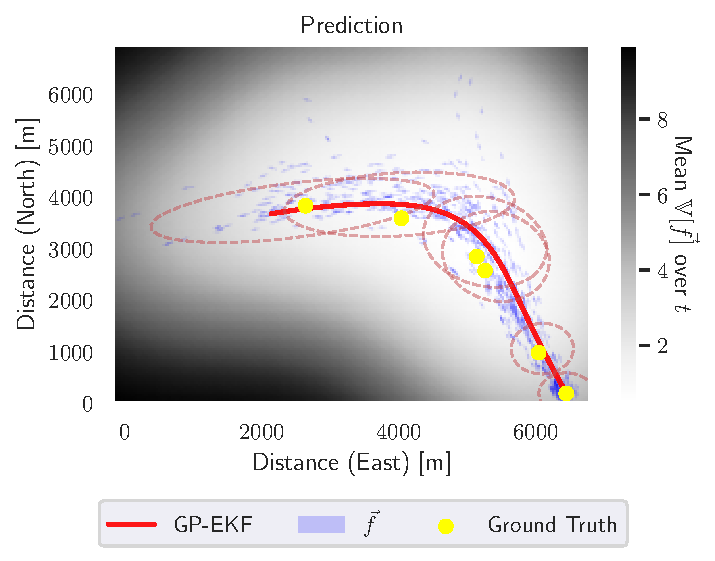
\includegraphics[width=\textwidth]{figures/dyngp/gp_ekf.pdf}
        \caption{Trajectory plotted against the vector-field $\vec{f}(\boldsymbol{x})$. The ellipses show the $95\%$ credibility interval for the predicted trajectory at the ground-truth timestamps.}
    \end{subfigure}
    \begin{subfigure}{\textwidth}
        \centering
        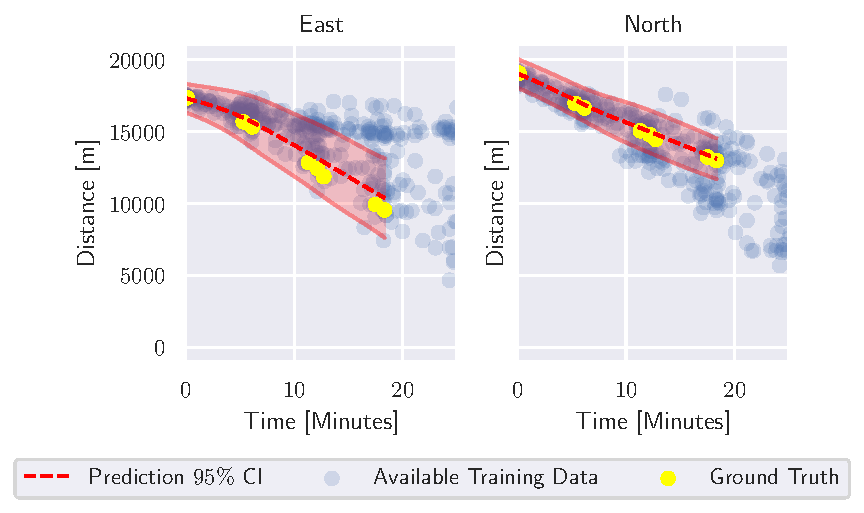
\includegraphics[width=\textwidth]{figures/dyngp/gp_ekf_state.pdf}
        \caption{$2\sigma$ credibility interval for the trajectory plotted against time}
    \end{subfigure}
    \caption{Predicted position using \cref{alg:gp_ekf_prediction}}
    \label{fig:gp_ekf}
\end{figure}


\section{Incorporating vessel position}
While the prediction procedure proposed in \cref{alg:gp_ekf_prediction} yields good predictions in many cases, it is inherently an open-loop prediction. Inaccurate predictions will never be corrected, propagating through any remaining iterations, potentially leading to significant errors later on. Looking at the available data in \cref{fig:gp_ekf_with_pdaf}, it would be desirable if the prediction converged towards available position measurements, \textit{slowly and only if the prediction is clearly wrong}. In other words, weak feedback compensating for minor prediction errors.

As no actual position measurements of the vessel's future position are available, the available training data are considered as \textbf{potential} measurements, which at any timestep may or may not originate from the vessel. Incorporating vessel position becomes a data association problem, for which one can look to target tracking for inspiration.

The \textit{\acrfull{pdaf}} is a method commonly used in target tracking which combines data association and filtering. The following introduction to \acrshort{pdaf} is mostly inspired by \cite{sensorfusjon}, with some adaptations to fit the current problem better. As single target tracking and data association is not the topic of this thesis, only a short introduction to the \acrshort{pdaf} will be included here. For more details, see \cite{sensorfusjon,bar1995multitarget}

In this section, all measurements in the available training set are considered as virtual \footnote{Virtual meaning a measurement that did not actually originate from the target vessel, but rather a measurement that could potentially originate from the target in the future. The word measurement is still used to keep the terminology similar to what is used by \acrshort{pdaf}.} position measurements, which may or may not originate from the vessel at time $t$. Similar to the \acrshort{pdaf}, it is assumed \textbf{at most one} measurement originating from the target to reduce the computational complexity significantly \cite{sensorfusjon}. As no proper measurements of the vessel's actual position, most of the measurements are assumed to be clutter, forcing the model to primarily trust its predictions.

Given the predicted state $\hat{\boldsymbol{x}}_t$, any real measurement is expected to be distributed around this state due to some measurement noise. Following the notation used by \acrshort{ekf}, and using the measurement model $h(\boldsymbol{x}) = \boldsymbol{x} \implies H = \frac{\partial h (\boldsymbol{x})}{\partial \boldsymbol{x}} = I$, the predicted measurement distribution is expressed as in \cref{eq:gp_ekf_pdaf_measurement} where the innovation covariance is defined as $\boldsymbol{S}_t \triangleq \hat{\boldsymbol{P}}_t + \boldsymbol{R}$ and $\boldsymbol{R}$ is the measurement noise.

\begin{equation} \label{eq:gp_ekf_pdaf_measurement}
    \hat{\boldsymbol{z}}_t \sim \mathcal{N}(\hat{\boldsymbol{x}}_t, \boldsymbol{S}_{t}) = \mathcal{N}(\hat{\boldsymbol{x}}_t, \hat{\boldsymbol{P}}_t + \boldsymbol{R})
\end{equation}

There is also the possibility that none of the measurements originated from the target, i.e., all observations are clutter. The choice of a good clutter model is a complicated topic, but the Poisson clutter model is used in this thesis. As the measurements are not actual measurements from the target, it is difficult to assign meaning to any clutter model. It, therefore, simply boils down to which parameters need to be tuned \footnote{The trajectory prediction is here considered to be target tracking of future position. The clutter parameters, therefore, need to be interpreted in the context of target tracking, not trajectory prediction.} and the Poisson clutter model should already be familiar to anyone with experience in target tracking.
According to the Poisson clutter model, the association probabilities are given by \cref{eq:pdaf_clutter_association_prob} \cite{sensorfusjon}, where $a_t$ is a discrete variable following a Categorical distribution where $a_t=k > 0$ denotes that measurement $k$ originated from the target. $a_t = 0$ is the special case when none of the measurements originated from the target, i.e., the predicted state should not be updated. $Z$ here denotes a matrix of all the measurements (positions) available in the training data and is independent of time, i.e., all measurements are always potential candidates. $\lambda$ denotes the clutter rate, and $P_D$ denotes the probability of detecting the target vessel.
\begin{equation}\label{eq:pdaf_clutter_association_prob}
    \Pr\{a_t | Z\} \propto \begin{cases}
        \lambda (1 - P_D)                                                                 & a_t = 0 \\
        P_D \mathcal{N} (\boldsymbol{z}^{a_t} | \hat{\boldsymbol{x}}_t, \boldsymbol{S}_t) & a_t > 0 \\
    \end{cases}
\end{equation}

Using the likelihood for each of the possible outcomes, the association probabilities $\boldsymbol{\beta}$ can be computed by normalizing the likelihood, i.e.

\begin{equation}
    \beta_i = \frac{\Pr\{a_t=i \; | \; Z\}}{\sum_{k=0}^M \Pr\{a_t=k \; | \; Z\}}
\end{equation}

The predicted state can then by updated using the Kalman update procedure for each the measurements individually. As the measurements $\boldsymbol{z}_t^{a_t > 0}$ are known values, the state innovation $\boldsymbol{v}_t^{a_t>0} \triangleq \boldsymbol{z}_t^{a_t>0} - \hat{\boldsymbol{z}}_t$ is distributed according to the measurement prediction $\hat{\boldsymbol{z}}_t$.

\begin{equation}
    \boldsymbol{v}_t^{a_t>0} \sim \mathcal{N}(\boldsymbol{z}_t^{a_t>0} - \hat{\boldsymbol{x}}_t, S_t)
\end{equation}
The updated state for each measurement is then given by the normal \acrshort{ekf} update step

\begin{equation}
    \boldsymbol{x}_t^{a_t > 0} = \hat{\boldsymbol{x}}_t + \boldsymbol{W}_t \boldsymbol{v}_t^{a_t > 0}
\end{equation} where $\boldsymbol{W}_t \triangleq \hat{\boldsymbol{P}}_t \boldsymbol{S}_t^{-1}$ is the Kalman gain.
The updated state of the vessel over all possible measurements can be described as a Gaussian Mixture Model over the $M+1$ different modes weighted by the association probabilites, i.e.
\begin{equation}
    p(\boldsymbol{x_t}) = \underbrace{\beta_0 \mathcal{N}(\boldsymbol{x}_t \; | \; \hat{\boldsymbol{x}}_t, \hat{\boldsymbol{P}}_t)}_{\text{No measurements are valid}} + \sum_{k=1}^M \underbrace{\beta_k \mathcal{N}\big(\boldsymbol{x}_t | \boldsymbol{x}_t^{a_k}, \boldsymbol{P}_t^{a_k}\big)}_{\text{Measurement $k$ is valid}}
\end{equation}


Moment reduction is then used to combined the different hypothesises into a single unimodal Gaussian distribution, i.e. a Gaussian distribution is fitted to the first and second moment (mean and variance) of the Gaussian mixture. The mean and variance of the resulting distribution is given by \cref{eq:pdaf_moment_mean} and \cref{eq:pdaf_moment_var} respectively, using $\boldsymbol{v}_t \triangleq \sum_{a_t > 0} \beta_t^{a_t} \boldsymbol{v}_t^{a_k}$.

\begin{subequations}
    \begin{align}
        \boldsymbol{x}_t & = \hat{\boldsymbol{x}}_t + \boldsymbol{W}_t \boldsymbol{v}_t \label{eq:pdaf_moment_mean} \\
        \begin{split}
            \boldsymbol{P}_t &= \hat{\boldsymbol{P}}_t - (1 - \beta_t^{0}) \boldsymbol{W}_t \boldsymbol{S}_t  \boldsymbol{W}_t\\ &+ \boldsymbol{W}_t \big[\sum_{a_t > 0}^M \beta_t^{a_t} \boldsymbol{v}_t^{a_t} (\boldsymbol{v}_t^{a_t})^\intercal - \boldsymbol{v}_t \boldsymbol{v}_t^\intercal \big] \boldsymbol{W}_t^\intercal\label{eq:pdaf_moment_var}
        \end{split}
    \end{align}
\end{subequations}

While available measurement could be used at each timestep, it is in practice more convenient only to include a subset which is close enough to the predicted state. As this measurement \textit{gate} should scale with the uncertainty, the gated subset is selected as \cref{eq:pdaf_gate} where $g$ is the number of standard deviations the method should consider.

\begin{equation} \label{eq:pdaf_gate}
    \mathcal{G} = \big\{ \boldsymbol{z} \; | \; (\boldsymbol{z} - \hat{\boldsymbol{x}}_t)^\intercal S^{-1} (\boldsymbol{z} - \hat{\boldsymbol{x}}_t) < g^2 \big\}
\end{equation}


By combining the \acrshort{pdaf} update with the GP-EKF prediction procedure in \cref{alg:gp_ekf_prediction}, the predicted trajectory can be tuned to favor areas with a large number of samples, effectively pulling the state towards areas with available samples. In regions with samples spread evenly around the predicted state, then the \acrshort{pdaf}'s effect is negligible (assuming proper tuning).

\begin{figure}
    \centering
    \begin{subfigure}{\textwidth}
        \centering
        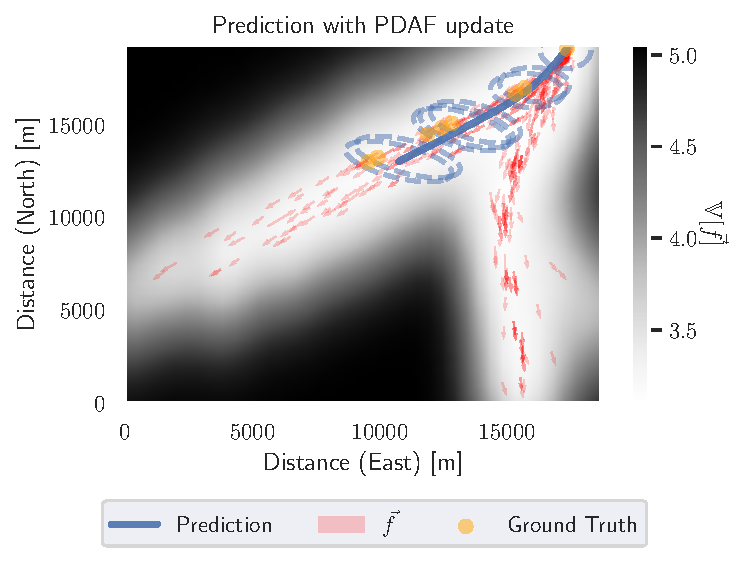
\includegraphics[width=\textwidth]{figures/dyngp/gp_ekf_with_pdaf.pdf}
        \caption{Trajectory plotted against the vector-field $\vec{f}(\boldsymbol{x})$. The ellipses show the $95\%$ credibility interval for the predicted trajectory at the ground-truth timestamps.}
    \end{subfigure}
    \begin{subfigure}{\textwidth}
        \centering
        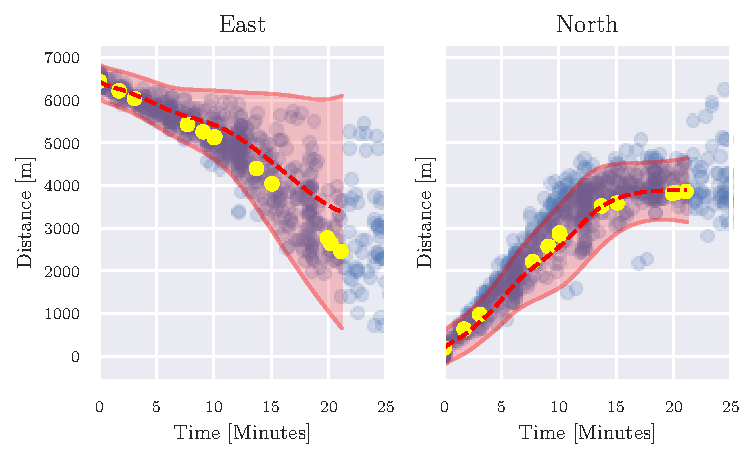
\includegraphics[width=\textwidth]{figures/dyngp/gp_ekf_with_pdaf_state.pdf}
        \caption{$95\%$ credibility interval for the trajectory plotted against time}
    \end{subfigure}
    \caption{Predicted position with the PDAF update procedure.}
    \label{fig:gp_ekf_with_pdaf}
\end{figure}

\subsection{Tuning PDAF parameters}
The model should primarily trust the prediction model, as it would otherwise get stuck as the measurements do not change over time. As the measurements do not originate from the target vessel, it is also expected to be a lot of noise in the measurements themselves. In practice, the tuning boils down to using a significant measurement noise $\boldsymbol{R}$ and a relatively low detection probability $P_D$ before tuning the clutter rate to achieve good results.

However, finding a set of parameters that works well across different trajectories turns out to be challenging. Parameters that improve the prediction for one trajectory may do more harm than good on another. The performance of using PDAF will be explored further in \cref{chap:stat_testing}.

\section{Implementation details}
This chapter has so far only discussed how $\vec{f}$ could be used to simulate trajectories. This section will discuss how the \acrshort{gp}s introduced in \cref{sec:gp} can be applied.

\subsection{Feature Engineering}
As $\vec{f}$ models the speed, rather than the position of the trajectories, the \acrshort{ais} needs some preprocessing before it can be used for training. There are two potential sources for the training samples $\boldsymbol{y}$:

\begin{enumerate}
    \item Trajectories from the dataset are converted into training samples for $\vec{f}$ using the simple first-order finite-difference method in \cref{eq:finite_difference} between subsequent \acrshort{ais} samples in a trajectory $i$. This yields the training outputs $\boldsymbol{y}_t^{i}$ corresponding to the inputs $\boldsymbol{\eta}_t^i$ such that $\boldsymbol{y}_t^i = \vec{f}(\boldsymbol{\eta}_t^i) + \epsilon$.
    \item The \acrshort{cog} and \acrshort{cog} from the \acrshort{ais} data can be used directly.
\end{enumerate}

\begin{align}\label{eq:finite_difference}
    \boldsymbol{y}_t = \frac{\boldsymbol{x}_{t+1} - \boldsymbol{x}_t}{\tau_{t+1} - \tau_t}
\end{align}


However, in practice, the dataset contains several contradicting trajectories. In a given area, vessels may move in opposite directions or with vastly different speeds. Therefore, the data needs to be filtered based on the relevance for the prediction, using the target vessel's position, \acrshort{cog} and \acrshort{sog} as decision parameters. The following pipeline is used to select relevant trajectories for training, given the vessel's current state:
\begin{enumerate}
    \item The distance between the target vessel and the initial position of the training trajectories must be less than $1000$ meters.
    \item The initial \acrshort{cog} of the training trajectories must be within $\pm 10^\circ$.
    \item The initial \acrshort{sog} of the training trajectories must be within $\pm 5$ knots.
\end{enumerate}


\subsection{Selecting a good kernel}
The kernel was, after trial and error, selected as the sum of three kernels. This kernel attempts to model the data as a combination of a long-term trend, dependent noise, and independent noise

\begin{equation}\label{eq:gp_ekf_kernel}
    k(\boldsymbol{\eta}_i, \boldsymbol{\eta}_j) = \sigma_0 k_0(\boldsymbol{\eta}_i, \boldsymbol{\eta}_j) + \sigma_1 k_1(\boldsymbol{\eta}_i, \boldsymbol{\eta}_j) +  \sigma_2 \delta(i, j)
\end{equation}

\begin{description}
    \item[Long term trend $k_0$] is a \acrshort{rbf} kernel intended to cover the long-term behavior of the trajectories, i.e., a smooth component describing the overall trend of the trajectories. The lengthscales of this kernel are assumed to be large.
    \item[Dependent noise $k_1$] is a \acrshort{rbf} kernel intended to model the variability between different trajectories not well explained by $k_0$. The lengthscales are assumed to be short.
    \item[Independent noise $\delta(i, j)$] is a white kernel intended to model any remaining error as \textit{\acrfull{iid}}.
\end{description}

\subsection{Optimizing the hyperparameters}
Independent lengthscales are used for each of the elements in $\boldsymbol{\eta}$, which in total yields $9$ hyperparameters to select. The hyperparameters are optimized using the \acrshort{ml} approach discussed in \cref{sec:gp_mle}. The implementation is readily available in the popular \textit{scikit-learn} \cite{scikit-learn} Python package. In order to avoid bad local optima, $10$ restarts with random initial conditions were used. After optimization, the parameters can be inspected to verify that the hyperparameters match our expectations.

\subsection{Alternative kernel choices}
Several other kernels were also attempted. The kernels were compared using the $R^2$ score for the test set in order to compare how well the \acrshort{gp} is able to express the variability between trajectories using different kernels.

\begin{description}
    \item[\acrshort{rbf} + \acrshort{iid} noise] was only able to express the long-term trend of the trajectories, but was unable to express uncertainty due to local variations. In practice, the optimization was unable to converge towards good hyperparameters, indicating an issue with the kernel specification.
    \item[\acrshort{rbf} + Matern + \acrshort{iid} noise] was tried with $\nu=\frac{1}{2}$, $\nu=\frac{3}{2}$ and $\nu=\frac{5}{2}$ without showing any benefits over the simpler \acrshort{rbf} based kernel in \cref{eq:gp_ekf_kernel}.
    \item[\acrshort{rbf} + Rational-Quadratic + \acrshort{iid}]
\end{description}

\section{Simulating trajectories using Gaussian Process Sequential Monte Carlo}
The Kalman-based prediction scheme proposed in the previous section works well as long as a single Gaussian distribution can sufficiently explain the uncertainty. However, in branching trajectories, minor differences in position early in the predicted trajectory might have significant effects on the following predictions. The result is a multimodal trajectory distribution, which a Kalman-based approach is not able to express.

Inspired by the prediction step used by \textit{particle filters} \cite{sensorfusjon}, the idea of sampling trajectories can be used to explore the multimodal trajectory distribution. While inspired by the particle filter, this approach will from now on be referred to as \textit{Sequential Monte-Carlo} to avoid confusion\footnote{An important part of the particle filter is weighting the particles based on available measurements. As only sampling of trajectories is performed, Sequential Monte-Carlo seems like a better fit.}. and to follow the same naming convention as used by \cite{pedestrian}.

The derivation of the Sequential Monte-Carlo approach is embarrassingly simple as this method trades high computational complexity for more straightforward mathematics. Instead of analytical propagation of uncertainty, many trajectories are simulated through random sampling and used to express the uncertainty empirically. The uncertainty for any trajectory distribution can be described, though at the cost of considerable computational complexity.
$N$ different trajectories are initialized with similar initial conditions. The trajectories are then simulated by drawing independent increments from $\vec{f}$ using the approach described in \cref{sec:gp_samples}, conditioned on the current state of each trajectory. The result is visualized in \cref{fig:gp_particle} for $N=500$ trajectories.
\begin{figure}[h]
    \centering
    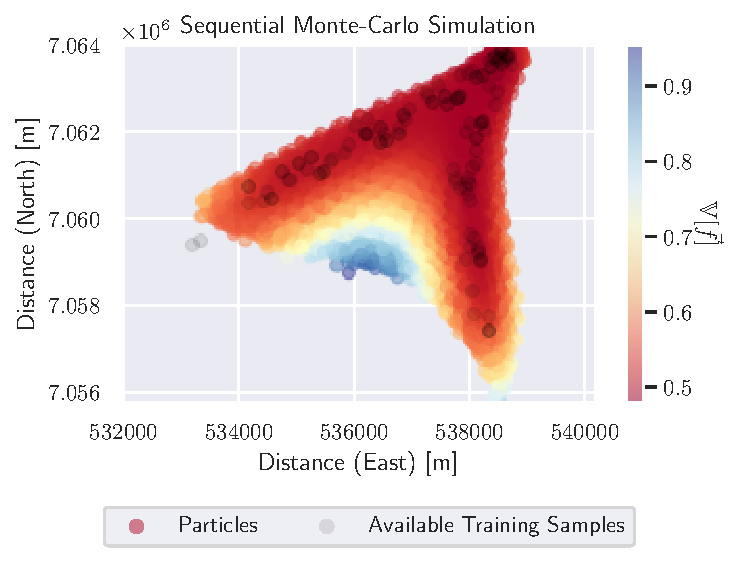
\includegraphics[width=\textwidth]{figures/dyngp/gp_particle.pdf}
    \caption{}
    \label{fig:gp_particle}
\end{figure}

\section{Other design choices}
\subsection{Why is $\vec{f}$ time-varying?}
The time component was initially included to handle trajectories with sharp turns better. If $\vec{f}$ only relied on position, the \acrshort{gp} would have no way of expressing that the speed vector at position $\boldsymbol{x}$ might change over time. The time component was later found to explain some of the variability in the velocity estimates, yielding better uncertainty estimates.

In practice, the \acrshort{ml} approach will, in many cases, yield very large lengthscales\footnote{In fact, the time lengthscale tends to reach a maximum value during optimization} for the time-components of the kernel, effectively disabling the time dependency. The time component is therefore only really used when the dataset contains a lot of time-dependent noise.

\subsection{Standardizing the training outputs $Y$}
\textit{Standardization}\todo[]{find source} is the process of converting the data into a standard unit of measurement, which in practice involves transforming the data to have zero mean and unit variance. This is useful when comparing measurements of different scales.

The proposed GP-EKF implementation works well with and without standardized input data, but standardization has one important benefit. While the current implementation allows separate kernel hyperparameters for each input dimension in $\boldsymbol{\eta}$, the kernel is assumed to be identical for each of the outputs in $\vec{f}$. The scale parameters $\sigma_i$ in the kernel therefore represents the variability of \textbf{both} output dimensions at once. However, with standardized training outputs $Y$, the scale parameters $\sigma_i$ are relative to the standard deviation of the training data. This way, the \acrshort{gp} can express different level of uncertianty for each output dimension, while still sharing the same kernel. Allowing separate kernels is a possible extensions, but is assumed to further complicate the hyperparameter selection.

\section{Summary}
This chapter has so far introduced a lot of new concepts, so that it might be nice with a summary of the overall pipeline:

\begin{enumerate}
    \item The raw \acrshort{ais} data is first grouped and sorted to get fixed-length trajectory vectors.
    \item Based on the target vessel's current state, such as position, \acrshort{cog} and \acrshort{sog}, trajectories with similar initial conditions is selected from the training set.
    \item Training inputs $\boldsymbol{\eta}$ and outputs $\boldsymbol{y}$ for $\vec{f}$ are generated from the training trajectories.
    \item The kernel hyperparameters are optimized using \acrshort{ml} in order to find the parameters which best explains the training data.
    \item The training data and kernel can then used to get the conditional distribution for $\vec{f}$.
    \item The \acrshort{ekf} procedure in \cref{alg:gp_ekf_prediction} is called repeatedly, using the current state of the target vessel as initial conditions. At each step, the \acrshort{pdaf} update procedure can be used as well if desired. Sequential Monte-Carlo can alternatively be used to simulate multimodal trajectories.
\end{enumerate}

The only parameters which need manual tuning are the time increment $\Delta \tau$ and the initial covariance $\boldsymbol{P}_0$. All other parameters are learned from the data.

